\chapter{Urban Source Identification Results and Discussion}

% https://e-reports-ext.llnl.gov/pdf/312592.pdf they show common false positive isotopes and we see a lot of overlap


\newcommand{\blackline}{\raisebox{2pt}{\tikz{\draw[-,black!40!black,solid,line width = 1.1pt](0,0) -- (6mm,0);}}}

\newcommand{\blackdotline}{\raisebox{2pt}{\tikz{\draw[-,black!40!black,dashed,line width = 1.1pt](0,0) -- (6mm,0);}}}

\newcommand{\blackdashdotline}{\raisebox{2pt}{\tikz{\draw[-,black!40!black,dash dot,line width = 1.1pt](0,0) -- (6mm,0);}}}

\newcommand{\blackdottedline}{\raisebox{2pt}{\tikz{\draw[-,black!40!black,dotted,line width = 1.1pt](0,0) -- (6mm,0);}}}

% \section{Problem Description and Training Dataset Overview}

This chapter applies machine learning algorithms to solve the problem of identifying a radioactive source in an urban environment. This scenario is applicable when performing source interdiction searching cargo containers, vehicles at boarder crossings, or surveying high profile events. 
% Urban environments present unique challenges to gamma-ray spectroscopy. Background radiation can change over city blocks due to different concentrations of uranium and thorium in building materials. Sources may be purposely shielded by unknown amounts of material to obscure their gamma-ray signal.





% \section{Data Augmentation Implementation}

% Because simulating a dataset with sufficient combinations of available data augmentation - seen in Tables \ref{table:all_fixed_simulation_parameters} and \ref{table:all_variable_simulation_parameters} - online data augmentation techniques are employed. Online data augmentation has the benefit of implicitly regularizing the models.

% Steps in the data augmentation process are:
% \begin{enumerate}
%   \item Randomly choose a background template with the same FWHM as the source template
%   \item Rebin source and background template with a random calibration
%   \item Apply the LLD to both templates
%   \item Normalize both templates by the sum of their respective counts 
%   \item Scale both signals by their respective total counts
%   \begin{itemize}
%      \item Counts defined by randomly chosen background counts per second, integration time, and signal to background ratio
%   \end{itemize}
%   \item Add both signals 
%   \item Poisson sample the resulting signal
% \end{enumerate}


\section{Learning Curve Analysis}

In this section we use learning curves to determine a sufficient number of training dataset examples for the simple and complete networks. To create the learning curves, a dataset of 3 x 10$^{8}$ spectra (1 x 10$^{4}$ examples per class) were generated for both the simple and complete dataset parameters (Tables \ref{table:hyperparameter_dataset_easy_parameters} and \ref{table:hyperparameter_dataset_full_parameters}). For each number of training examples, five random subsets of the total spectra were used as training sets. Stratified sampling was used to keep the number of examples per class in each subset as equal as possible. A separate holdout dataset of 300 total spectra (10 examples per class) was used as a testing dataset set. Training was ended after an early stopping condition with a patience of 100 epochs was reached.

Figure \ref{fig:learning_curves_easy} shows the learning curves for each simple model's F1 score asymptotes to one past 5000 examples. This shows that each model is well suited to generalize within the simple parameter space. Training was rerun on one CAE model at 1 x 10$^{4}$ and 2 x 10$^{4}$ samples due to the error not decreasing during training. This can be attributed to a poor CAE pretraining.


\begin{figure}[H]
	\centering
	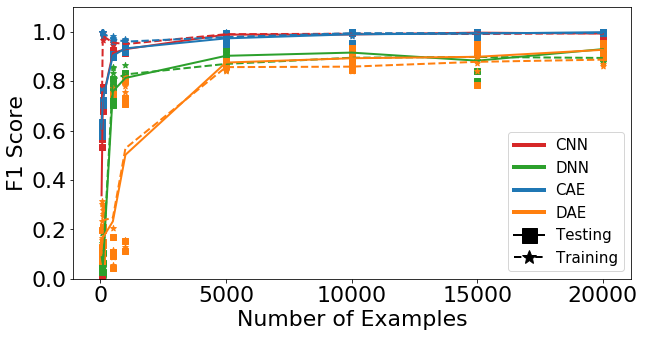
\includegraphics[width=0.9\linewidth]{images/learning_curves_easy}
	\caption{Learning curves for each simple model.}
	\label{fig:learning_curves_easy}
\end{figure}


The testing set error curves in Figure \ref{fig:learning_curves_full} are less steep than those in the simple learning curve plot. This shows that the patterns in the complete dataset are more complex and models require more examples to generalize to unseen complete dataset examples. The learning curve for the complete model shows the CNN and DNN converging to near one after 5 x 10$^{3}$ and 1.5 x 10$^{4}$ examples. The testing and training F1 score curves for the CNN and DNN also show low-bias and low-variance, indicating the hyperparameter search found appropriate values for the complexity of the complete dataset.

The training errors for the autoencoder models do not saturate as quickly as the training errors for the CNN and DNN. This shows that either the pretraining has a large effect on learning or the pretrained models need regularization during fine-tuning. Both the DAE and CAE saturate past 1 x 10$^{4}$ examples. Similar to the simple training curve, training was rerun on one CAE model at 1.5 x 10$^{4}$ and 2 x 10$^{4}$.



\begin{figure}[H]
	\centering
	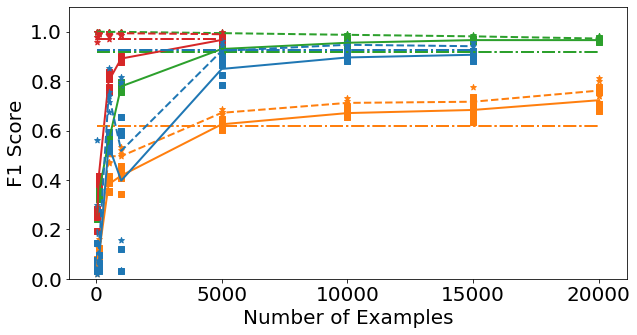
\includegraphics[width=0.9\linewidth]{images/learning_curves_full}
	\caption{Learning curves for each complete model.}
	\label{fig:learning_curves_full}
\end{figure}



\section{Generalization Performance Evaluation}

In this section we analyze the generalization performance of each machine learning model and the simple and complete training datasets. To quantify performance on a range of spectral qualities, the F1-scores are averaged for each model trained on a dataset of 10000 examples. Testing data are simulated over integration times log-uniformly sampled from one seconds to an hour and signal to background ratios of 0.1 and 0.5. Default simulation parameters are shown in Table \ref{table:default_sim_params}. Changes to these defaults are indicated for each generalization experiment. To reduce variance, ten spectra are generated for each isotope and simulated parameter combination. Models trained on the simple and complete datasets are referred to as simple models and complete models.

\begin{table}[H]
\centering
\caption{Default parameters used for all generalization datasets.}
\label{table:default_sim_params}
\begin{tabular}{ll}
% \cline{2-3}
\hline
\textbf{Simulation Parameter} &  \textbf{Value} \\ \hline
Source-Detector Distance [cm] & 175.0\\ 
Source-Detector Height [cm] & 100.0\\ 
FWHM 662 keV [s] & 7.0\\ 
Shielding [\% 200 keV Attenuated] & 0\% \\ 
Calibration - Offset [channels] & 0 \\ 
Calibration - Gain & 1.0 \\ 
Background Counts Per Second & 200 \\ \hline 
\end{tabular}
\end{table}


% \begin{figure}[H]
%      \centering
%      \begin{subfigure}[b]{0.49\textwidth}
%          \centering
%          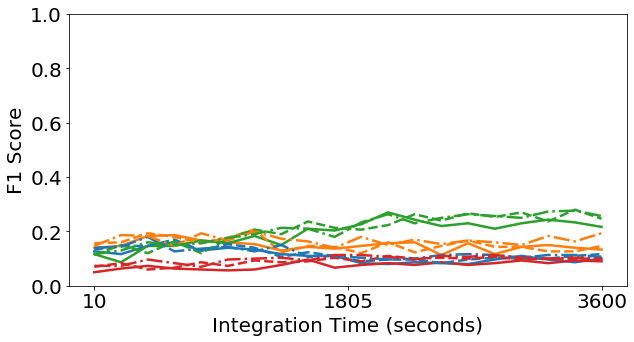
\includegraphics[width=\textwidth]{images/generalization-height-easy-01.png}
%          \caption{}
%          \label{fig:generalization-height-easy-01}
%      \end{subfigure}
%      \hfill
%      \begin{subfigure}[b]{0.49\textwidth}
%          \centering
%          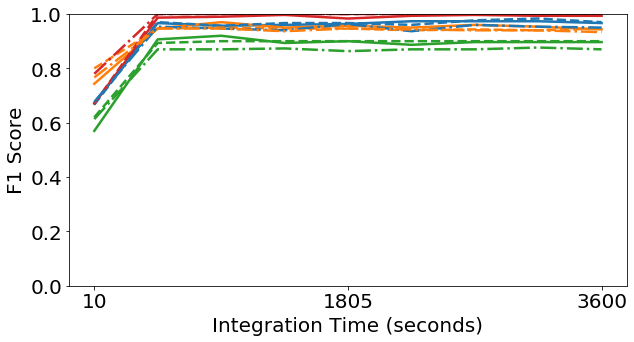
\includegraphics[width=\textwidth]{images/generalization-height-easy-05.png}
%          \caption{}
%          \label{fig:generalization-height-easy-05}
%      \end{subfigure}

%         \caption{Examples of spectra simulated with different signal-to-background ratios,}
%         \label{fig:generalization_signalbackground_examples}
% \end{figure}


% When the error between models differs significantly or is particularly large, confusion matrices are included to show what isotopes are problematic.


\subsection{Generalization Performance on Source-Detector Height}

In this section we analyze the generalization performance of each network on changes in source-detector height off the ground. This tests if each model is sensitive to changes in the Compton continuum due to environmental scattering associated with the source-detector height. An example of these changes can be seen in Figure \ref{fig:sim_spectra_height_comparison}.

As seen in Figure \ref{fig:generalization_height_fixeddataset}, the performance of each network was not significantly changed with changes to source-detector height. This shows that performance is not impacted by the relatively small changes in the Compton continuum caused by varying the source-detector height. Each CNN - except the simple CNN identifying the lower signal-to-background ratio spectra - had the highest F1 score. Figure \ref{fig:generalization-height-easy-05} also shows that the simple dataset generalized to changes in source-detector height in higher signal-to-background ratio spectra. The complete DAE performed particularly poorly while the complete CAE and DNN performed similarly.
% , indicating that either the pretraining produced a poor encoding that was difficult to fine-tune through further training.

Models trained on the simple dataset did not generalize well to low signal-to-background data, shown in \ref{fig:generalization-height-easy-01}. The simple DNN outperformed the other models in this dataset. This is consistent with the thought that the DNN is using a ROI approach to identification and the CNN is using more abstract features. The scale of abstract features (like those associated with the Compton continuum) are different at a signal-to-background ratio of 0.1 compared to 0.5. This difference makes the features used by the simple CNN different from those required by the complete CNN.


\begin{figure}[H]
     \centering
     \begin{subfigure}[b]{0.49\textwidth}
         \centering
         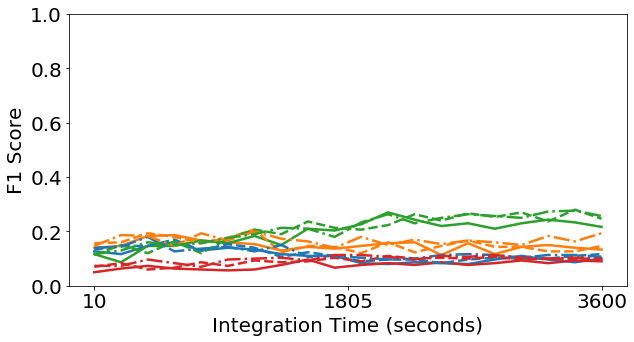
\includegraphics[width=\textwidth]{images/generalization-height-easy-01.png}
         \caption{}
         \label{fig:generalization-height-easy-01}
     \end{subfigure}
     \hfill
     \begin{subfigure}[b]{0.49\textwidth}
         \centering
         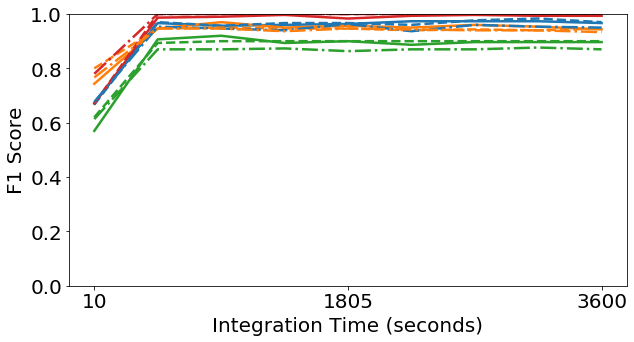
\includegraphics[width=\textwidth]{images/generalization-height-easy-05.png}
         \caption{}
         \label{fig:generalization-height-easy-05}
     \end{subfigure}

     \begin{subfigure}[b]{0.49\textwidth}
         \centering
         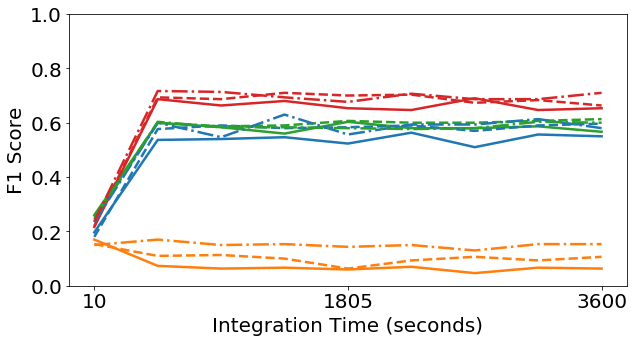
\includegraphics[width=\textwidth]{images/generalization-height-full-01.png}
         \caption{}
         \label{fig:generalization-height-full-01}
     \end{subfigure}
     \hfill
     \begin{subfigure}[b]{0.49\textwidth}
         \centering
         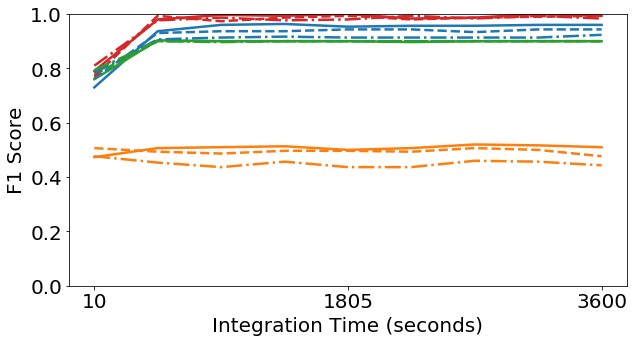
\includegraphics[width=\textwidth]{images/generalization-height-full-05.png}
         \caption{}
         \label{fig:generalization-height-full-05}
     \end{subfigure}
    % \begin{tabular}{r@{: }l r@{: }l}
    \begin{tabular}{r@{: }l r@{: }l r@{: }l r@{: }l}
    DNN & Green & CNN & Red & DAE & Yellow & CAE & Blue\\
    \end{tabular}
    \begin{tabular}{r@{: }l r@{: }l r@{: }l}
    50 cm & \blackline & 100 cm & \blackdotline & 150 cm & \blackdashdotline
    \end{tabular}
    
        \caption{Each model's generalization performance with respect to the height-off-ground parameter. Networks were trained with a fixed-size dataset. Figures in the top and bottom row are trained using the simple and complete dataset and Figures in the first and second column are use spectra with signal-to-background ratios of 0.1 and 0.5, respectively.}
        \label{fig:generalization_height_fixeddataset}
\end{figure}


\subsection{Generalization Performance on Source-Detector Standoff Distance}

In this section we analyze the generalization performance of each network on changes in source-detector standoff distance. This tests if each model is sensitive to larger changes in the Compton continuum compared to those associated with changes in source-detector height. An example of these changes can be seen in Figure \ref{fig:sim_spectra_distance_comparison}.

As seen in Figure \ref{fig:generalization_dist_fixeddataset}, general trends seen in the source-detector height generalization, such as superior performance of the CNN and the poor DAE encoding, are observed in source-detector distance generalization. Changing the source-detector distance changes performance more noticeably compared to changes in standoff distance. This was especially noticeable for the shorter standoff distance of 50 cm. At this distance, the peak-to-total ratio increases significantly, which emphasizes the peak information while reducing the Compton continuum. At the lower signal-to-background ratio the closer standoff distance improves performance in each network while at the higher signal-to-background ratio this trend is reversed. A higher peak-to-total ratio makes identification easier for algorithms that focus on photopeaks. The reduced performance of each model on high peak-to-total ratio spectra on the higher signal-to-background data shows performance expected from a template matching or pattern recognition algorithm.
% that the models are acting more similarly to a  than a ROI approach. 


\begin{figure}[H]
     \centering
     \begin{subfigure}[b]{0.49\textwidth}
         \centering
         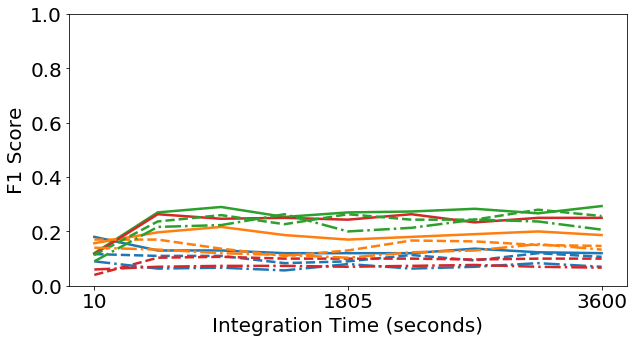
\includegraphics[width=\textwidth]{images/generalization-dist-easy-01.png}
         \caption{}
         \label{fig:generalization-dist-easy-01}
     \end{subfigure}
     \hfill
     \begin{subfigure}[b]{0.49\textwidth}
         \centering
         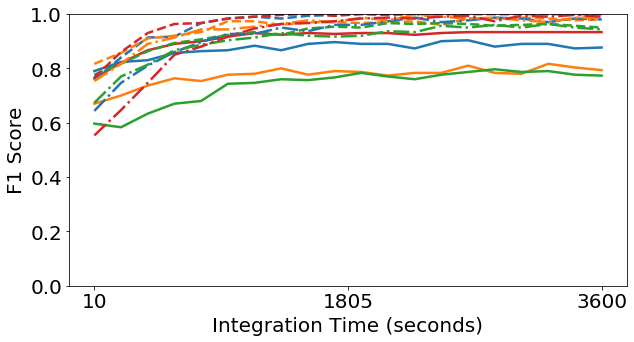
\includegraphics[width=\textwidth]{images/generalization-dist-easy-05.png}
         \caption{}
         \label{fig:generalization-dist-easy-05}
     \end{subfigure}

     \begin{subfigure}[b]{0.49\textwidth}
         \centering
         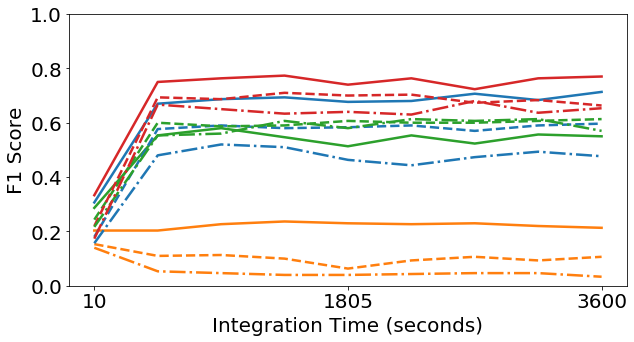
\includegraphics[width=\textwidth]{images/generalization-dist-full-01.png}
         \caption{}
         \label{fig:generalization-dist-full-01}
     \end{subfigure}
     \hfill
     \begin{subfigure}[b]{0.49\textwidth}
         \centering
         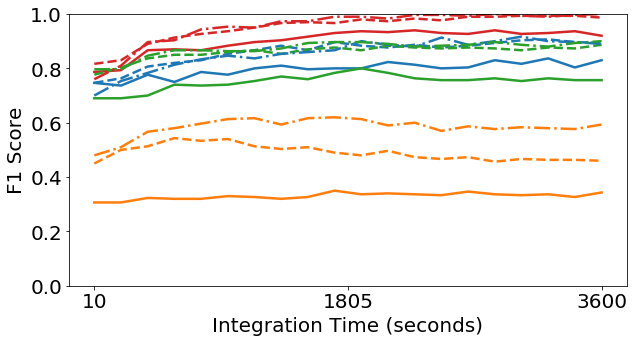
\includegraphics[width=\textwidth]{images/generalization-dist-full-05.png}
         \caption{}
         \label{fig:generalization-dist-full-05}
     \end{subfigure}
    \begin{tabular}{r@{: }l r@{: }l r@{: }l r@{: }l}
    DNN & Green & CNN & Red & DAE & Yellow & CAE & Blue\\
    \end{tabular}
    \begin{tabular}{r@{: }l r@{: }l r@{: }l}
    50 cm & \blackline & 175 cm & \blackdotline & 300 cm & \blackdashdotline
    \end{tabular}
        \caption{Each model's generalization performance with respect to the source-detector distance parameter. Networks were trained using fixed-size datasets. Figures in the top and bottom row are trained using the simple and complete dataset and Figures in the first and second column are use spectra with signal-to-background ratios of 0.1 and 0.5, respectively.}
        \label{fig:generalization_dist_fixeddataset}
\end{figure}




\subsection{Generalization Dependence on Resolution}

In this section we analyze the generalization performance of each network on changes in detector resolution. An example of these changes can be seen in Figure \ref{fig:sim_spectra_FWHM_comparison}.

Changes in resolution do not significantly impact performance of the models. General trends are similar to distance and height generalization.


\begin{figure}[H]
     \centering
     \begin{subfigure}[b]{0.49\textwidth}
         \centering
         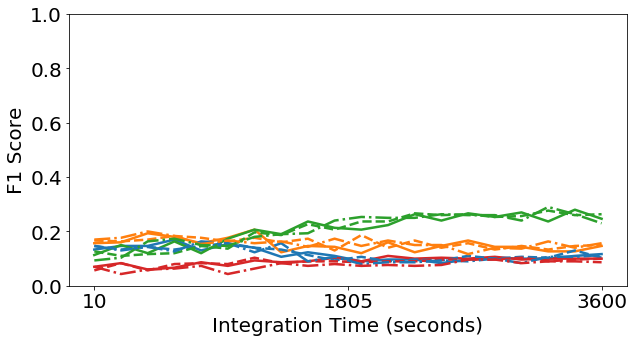
\includegraphics[width=\textwidth]{images/generalization-fwhm-easy-01.png}
         \caption{}
         \label{fig:generalization-fwhm-easy-01}
     \end{subfigure}
     \hfill
     \begin{subfigure}[b]{0.49\textwidth}
         \centering
         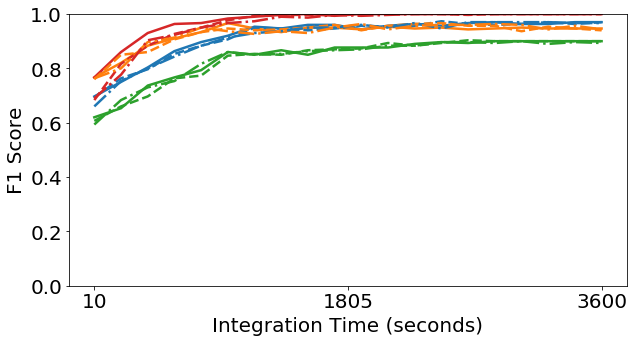
\includegraphics[width=\textwidth]{images/generalization-fwhm-easy-05.png}
         \caption{}
         \label{fig:generalization-fwhm-easy-05}
     \end{subfigure}

     \begin{subfigure}[b]{0.49\textwidth}
         \centering
         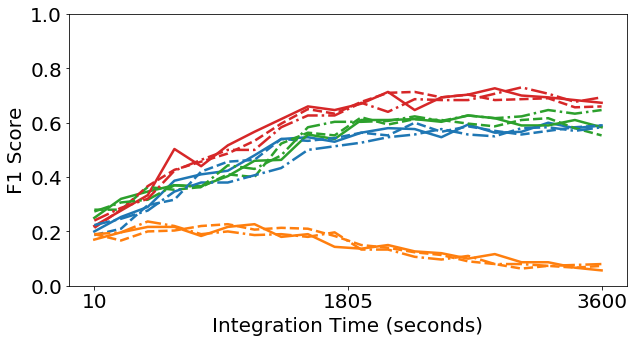
\includegraphics[width=\textwidth]{images/generalization-fwhm-full-01.png}
         \caption{}
         \label{fig:generalization-fwhm-full-01}
     \end{subfigure}
     \hfill
     \begin{subfigure}[b]{0.49\textwidth}
         \centering
         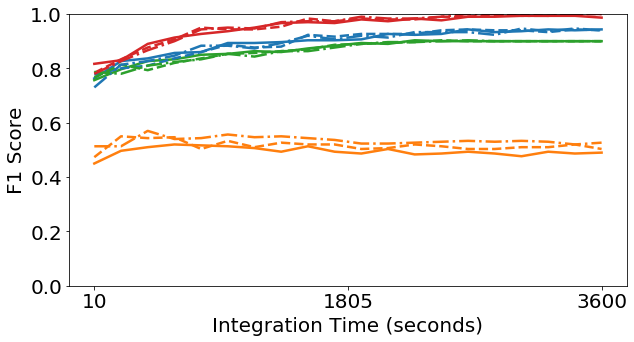
\includegraphics[width=\textwidth]{images/generalization-fwhm-full-05.png}
         \caption{}
         \label{fig:generalization-fwhm-full-05}
     \end{subfigure}
    \begin{tabular}{r@{: }l r@{: }l r@{: }l r@{: }l}
    DNN & Green & CNN & Red & DAE & Yellow & CAE & Blue\\
    \end{tabular}
    \begin{tabular}{r@{: }l r@{: }l r@{: }l}
    7.0 & \blackline & 7.5 & \blackdotline & 8.0 & \blackdashdotline
    \end{tabular}
        \caption{Each model's generalization performance with respect to the detector resolution. Networks were trained using fixed-size datasets. Resolutions in legend are measured at 662 keV. Figures in the top and bottom row are trained using the simple and complete dataset and Figures in the first and second column are use spectra with signal-to-background ratios of 0.1 and 0.5, respectively.}
        \label{fig:generalization_fwhm_fixeddataset}
\end{figure}


\subsection{Generalization Dependence on Shielding.}

In this section we analyze the generalization performance of each network on changes in shielding. Spectra were simulated with iron shielding that shields 40\%, 60\%, and 80\% of the intensity of a 200 keV gamma-ray.

As seen previously, simple models do not generalize to the lower signal-to-background spectra. Simple models, which only uses unshielded and 20\% shielded templates, do generalize to other shielding thicknesses in higher signal-to-background spectra. Each simple model achieves and F1 score above 80\% after 2000 seconds for the 40\% attenuated spectra. Only the CAE achieves similar performance for the 40\% attenuated spectra. All other models and shielding settings attain F1 scores between 50\% and 75\%.

The complete models perform better in the low signal-to-background spectra. Both complete convolutional models perform comparatively and outperform the complete dense models. Each network's performance on 40\% and 60\% attenuated spectra were comparable, while the 80\% attenuation reduced performance more significantly. Similar trends are seen in higher signal-to-background spectra. 


\begin{figure}[H]
     \centering
     \begin{subfigure}[b]{0.49\textwidth}
         \centering
         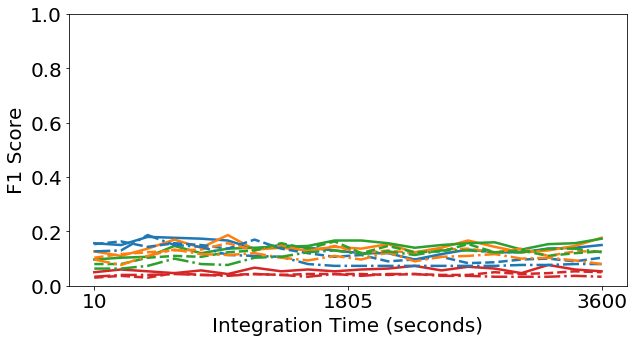
\includegraphics[width=\textwidth]{images/generalization-shielding-easy-01.png}
         \caption{}
         \label{fig:generalization-shielding-easy-01}
     \end{subfigure}
     \hfill
     \begin{subfigure}[b]{0.49\textwidth}
         \centering
         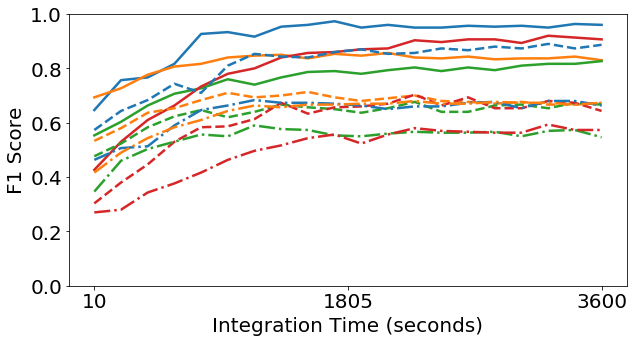
\includegraphics[width=\textwidth]{images/generalization-shielding-easy-05.png}
         \caption{}
         \label{fig:generalization-shielding-easy-05}
     \end{subfigure}

     \begin{subfigure}[b]{0.49\textwidth}
         \centering
         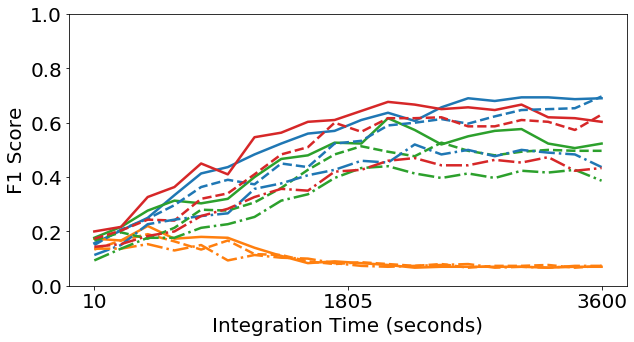
\includegraphics[width=\textwidth]{images/generalization-shielding-full-01.png}
         \caption{}
         \label{fig:generalization-shielding-full-01}
     \end{subfigure}
     \hfill
     \begin{subfigure}[b]{0.49\textwidth}
         \centering
         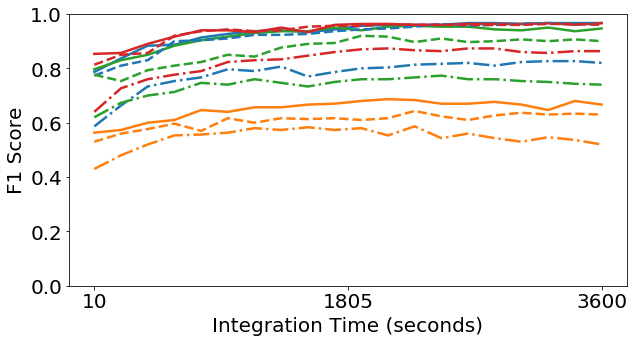
\includegraphics[width=\textwidth]{images/generalization-shielding-full-05.png}
         \caption{}
         \label{fig:generalization-shielding-full-05}
     \end{subfigure}
    \begin{tabular}{r@{: }l r@{: }l r@{: }l r@{: }l}
    DNN & Green & CNN & Red & DAE & Yellow & CAE & Blue\\
    \end{tabular}
    \begin{tabular}{r@{: }l r@{: }l r@{: }l}
    40\% & \blackline & 60\% & \blackdotline & 80\% & \blackdashdotline
    \end{tabular}
    
    
        \caption{Shielding generalization performance of each model trained using a fixed dataset. Figures in the top and bottom row are trained using the simple and complete dataset and Figures in the first and second column are use spectra with signal-to-background ratios of 0.1 and 0.5, respectively.}
        \label{fig:generalization_shielding_fixeddataset}
\end{figure}


Performance in data augmented models was similar to the fixed dataset models at the lower signal-to-background ratio and simple dataset. At the higher signal-to-background ratio performance dropped, especially for the CAE whose F1 score was near zero throughout the range of integration times. This shows that the CAE overtrained to the patterns in the simple dataset and did not generalize to new shielding configurations.

Performance for the data augmented models on data simulated with complete parameters was similar to the fixed dataset models at the low signal-to-background ratio and comparable at the higher signal-to-background ratio. The main difference was the improved performance of the complete CNN at the lower signal-to-background ratio.



\begin{figure}[H]
     \centering
     \begin{subfigure}[b]{0.49\textwidth}
         \centering
         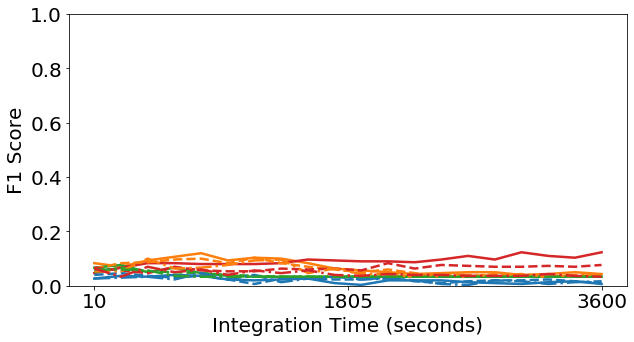
\includegraphics[width=\textwidth]{images/generalization-shielding-aug-easy-01.png}
         \caption{}
         \label{fig:generalization-shielding-aug-easy-01}
     \end{subfigure}
     \hfill
     \begin{subfigure}[b]{0.49\textwidth}
         \centering
         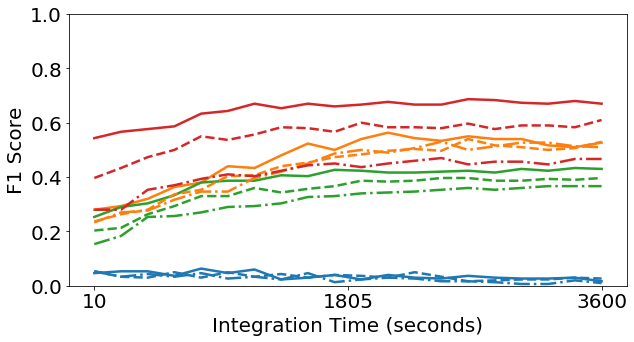
\includegraphics[width=\textwidth]{images/generalization-shielding-aug-easy-05.png}
         \caption{}
         \label{fig:generalization-shielding-aug-easy-05}
     \end{subfigure}

     \begin{subfigure}[b]{0.49\textwidth}
         \centering
         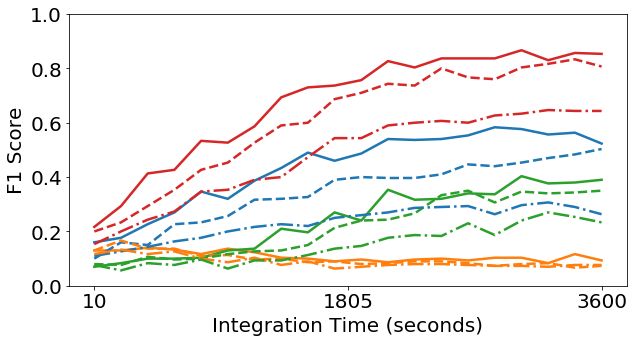
\includegraphics[width=\textwidth]{images/generalization-shielding-aug-full-01.png}
         \caption{}
         \label{fig:generalization-shielding-aug-full-01}
     \end{subfigure}
     \hfill
     \begin{subfigure}[b]{0.49\textwidth}
         \centering
         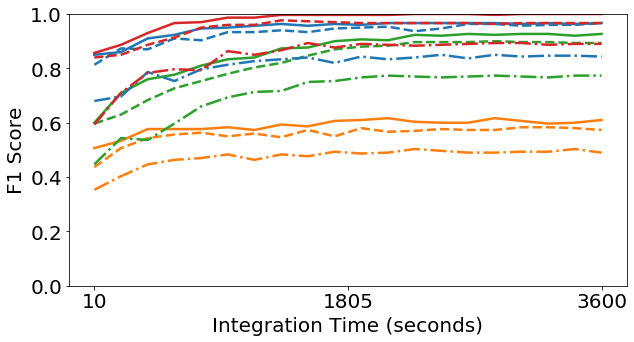
\includegraphics[width=\textwidth]{images/generalization-shielding-aug-full-05.png}
         \caption{}
         \label{fig:generalization-shielding-aug-full-05}
     \end{subfigure}
    \begin{tabular}{r@{: }l r@{: }l r@{: }l r@{: }l}
    DNN & Green & CNN & Red & DAE & Yellow & CAE & Blue\\
    \end{tabular}
    \begin{tabular}{r@{: }l r@{: }l r@{: }l}
    40\% & \blackline & 60\% & \blackdotline & 80\% & \blackdashdotline
    \end{tabular}
        \caption{Shielding generalization performance of each model trained using data augmentation, Figures in the top and bottom row are trained using the simple and complete dataset and Figures in the first and second column are use spectra with signal-to-background ratios of 0.1 and 0.5, respectively.}
        \label{fig:generalization_shielding_augdataset}
\end{figure}



\subsection{Generalization Dependence on Gain}

In this section we analyze the generalization performance of each network on changes in calibration. Spectra were simulated with relative calibration gains of 0.8, 1.0, and 1.2. The 1.0 gain setting calibrates the 1024$^{th}$ channel of the spectrum to 3 Mev.

At the higher signal-to-background ratio the simple models begin generalizing to the 1.2 relative gain while performing poorly on the 0.8 relative gain. The lower relative gain has the potential to push spectral features into the LLD, removing them from the signal. Because the simple dataset parameters never obscure these features, the simple models cannot correctly identify spectra without them.

The complete models performed better with changing gain, but still struggled with the 0.8 relative gain.  Compared to other complete models, the complete CNN performed the best on each relative gain setting.


\begin{figure}[H]
     \centering
     \begin{subfigure}[b]{0.49\textwidth}
         \centering
         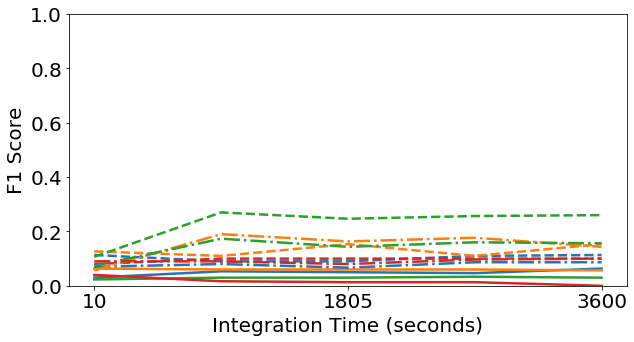
\includegraphics[width=\textwidth]{images/generalization-cal-easy-01.png}
         \caption{}
         \label{fig:generalization-cal-easy-01}
     \end{subfigure}
     \hfill
     \begin{subfigure}[b]{0.49\textwidth}
         \centering
         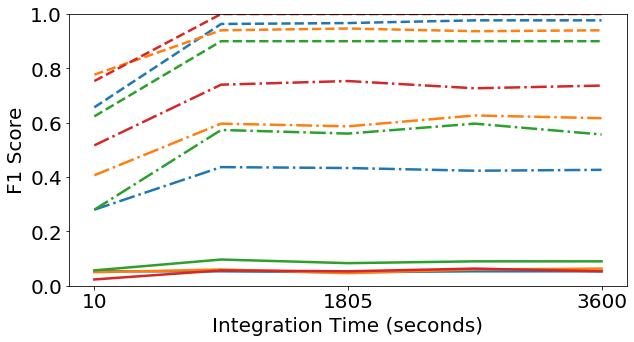
\includegraphics[width=\textwidth]{images/generalization-cal-easy-05.png}
         \caption{}
         \label{fig:generalization-cal-easy-05}
     \end{subfigure}

     \begin{subfigure}[b]{0.49\textwidth}
         \centering
         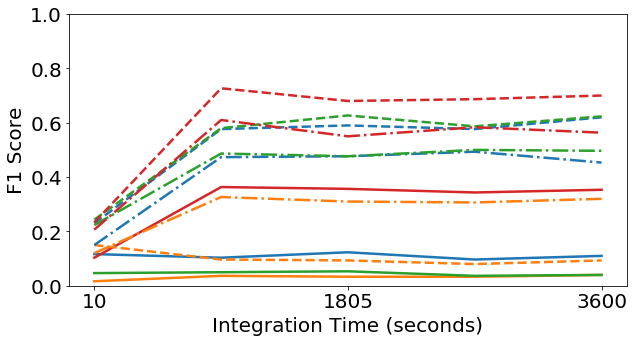
\includegraphics[width=\textwidth]{images/generalization-cal-full-01.png}
         \caption{}
         \label{fig:generalization-cal-full-01}
     \end{subfigure}
     \hfill
     \begin{subfigure}[b]{0.49\textwidth}
         \centering
         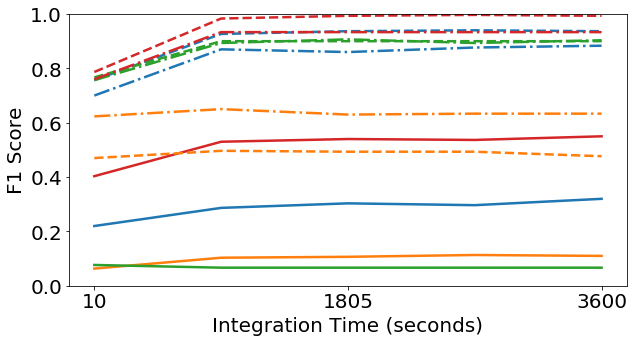
\includegraphics[width=\textwidth]{images/generalization-cal-full-05.png}
         \caption{}
         \label{fig:generalization-cal-full-05}
     \end{subfigure}
    \begin{tabular}{r@{: }l r@{: }l r@{: }l r@{: }l}
    DNN & Green & CNN & Red & DAE & Yellow & CAE & Blue\\
    \end{tabular}
    \begin{tabular}{r@{: }l r@{: }l r@{: }l}
    0.8 & \blackline & 1.0 & \blackdotline & 1.2 & \blackdashdotline
    \end{tabular}
        \caption{Calibration gain generalization performance of each model trained using a fixed dataset. Figures in the top and bottom row are trained using the simple and complete dataset and Figures in the first and second column are use spectra with signal-to-background ratios of 0.1 and 0.5, respectively.}
        \label{fig:generalization_cal_fixeddataset}
\end{figure}


% \subsection{Generalization Dependence on Changing Background.}

% Datasets were simulated with backgrounds different from the training set and real measured background. It is expected that the complete dataset will mistake background for isotopes more often than the simplified dataset because photopeaks are decreased by shielding.


% \subsection{Results on Spectra for ANSI compliance}

% This section shows model asymptotic performance vs integration time for ANSI compliance. Using N models (justified previously as asymptotic). 



% \begin{table}[H]
% \centering
% \caption{Isotope combinations required for the ANSI standard \cite{ANSI}.}
% \begin{tabular}{c}
% Isotope Combinations \\ \hline
% $^{137}$Cs + depleted uranium (DU) \\ % \hline
% $^{99m}$Tc + HEU \\ % \hline
% $^{201}$Tl + HEU \\ % \hline
% $^{67}$Ga + HEU \\ % \hline
% $^{131}$I + WGPu \\ % \hline
% NORM + HEU \\ % \hline
% NORM + WGPu \\ % \hline
% \end{tabular}
% \end{table}



% \begin{figure}[H]
%      \centering
%      \begin{subfigure}[b]{0.9\textwidth}
%          \centering
%          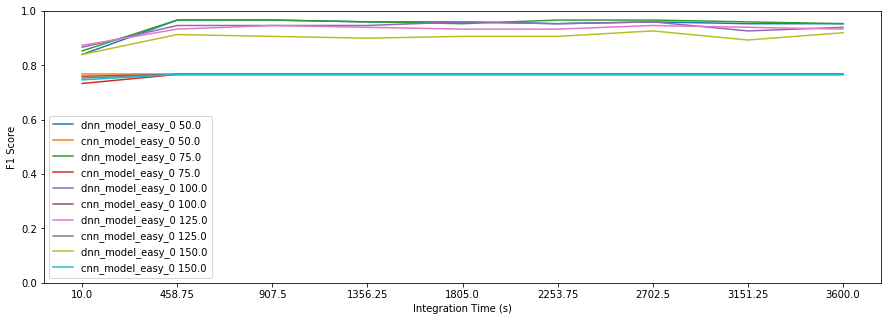
\includegraphics[width=\textwidth]{images/results_easy_distance_comparison}
%          \caption{Simplified Dataset.}
%          \label{fig:results_full_background_inject_simple}
%      \end{subfigure}

%      \begin{subfigure}[b]{0.9\textwidth}
%          \centering
%          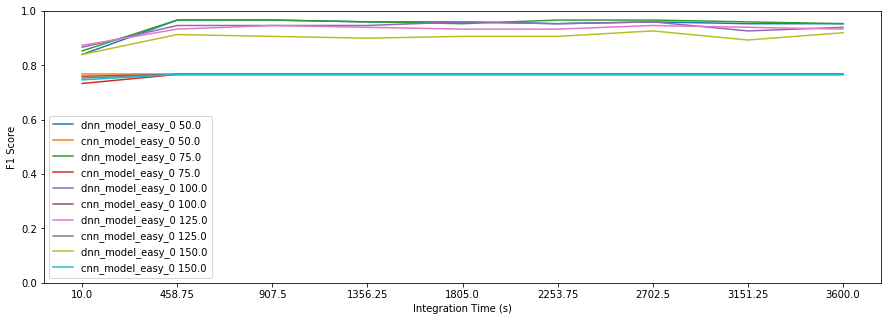
\includegraphics[width=\textwidth]{images/results_easy_distance_comparison}
%          \caption{Complete Dataset.}
%          \label{fig:results_full_background_inject_full}
%      \end{subfigure}

%         \caption{F1 score for models tested on ANSI isotope combinations.}
%         \label{fig:results_full_background_inject}
% \end{figure}



\subsection{Results on Measured Spectra}

This section shows performance over integration time for different calibration settings and shielding amounts in real gamma-ray spectra. Sources include $^{137}$Cs, $^{60}$Co, $^{133}$Ba, and $^{152}$Eu. A diagram of the laboratory setup used for these measurements is shown in Figure \ref{fig:shielding_measurment_diagram}. The radioactive sources, 1 inch diameter by 1/8 inch thick plastic disks containing radioactive material, were measured on a wooden desk approximately one meter from the nearest wall to reduce radiation backscatter. We used a 2x2 inch Ortec NaI detector to measure the sources. Blocks of shielding material were added for the measurements in Section \ref{real_shielding_performance}. Measurements in Section \ref{real_calibration_performance} used no shielding material.

\begin{figure}[H]
	\centering
	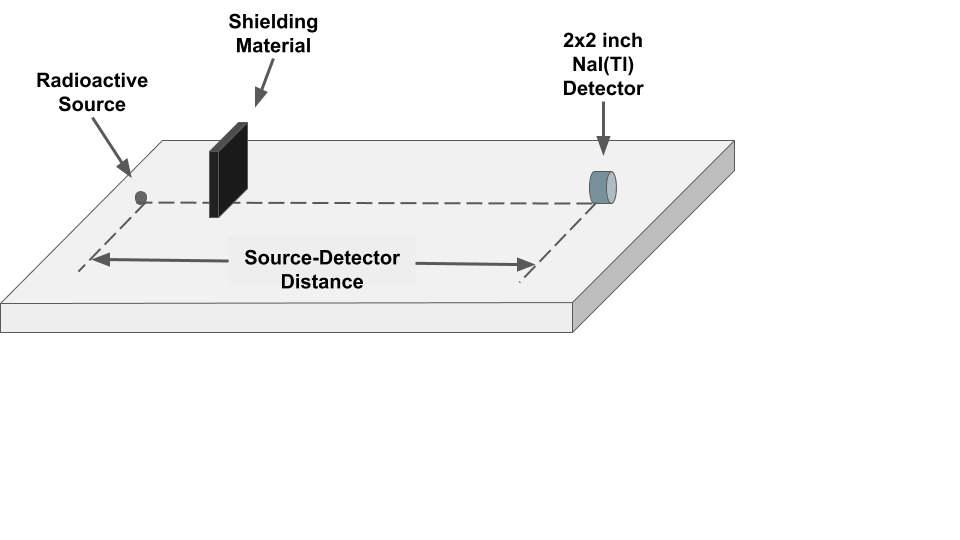
\includegraphics[trim=0 200 210 0,clip,width=0.9\linewidth]{images/shielding_measurment_diagram}
	\caption{Diagram of the laboratory setup used to measure radioactive sources.}
	\label{fig:shielding_measurment_diagram}
\end{figure}


\subsubsection{Asymptotic Model Performance on Changing Voltage} \label{real_calibration_performance}

To test the dependence of performance of each model to changes in calibration, spectra with different voltages were recorded and the posterior probability of the measured isotope found by each model is observed over integration time. The detector's calibrations was varied by changing the PMT voltage to 720 V, 745 V, 770 V, and 795 V. The detector calibration of 770 V calibrated the detector's 1024$^{th}$ channel to 3 MeV. Reported relative gain settings are calibrated to the 662 keV photopeak defining the 770 V calibration as the reference. Sources measured include $\mu$Ci level $^{137}$Cs, $^{60}$Co, $^{152}$Eu, and $^{133}$Ba. The standoff distance of each source was adjusted to keep the counts-per-second from the source equal-to and one-half-of the counts-per-second from background.

The figures in \ref{fig:gain_cs137} show trained ANN performance when identifying $^{137}$Cs. Models trained on the simple dataset, Figures \ref{fig:realspectra-cal-cs137-0-easy} and \ref{fig:realspectra-cal-cs137-1-easy}, did not generalize well to calibrations outside the training set. When trained on both the simple and complete dataset, The CNN performed well. Both CNNs identified $^{137}$Cs with a 100\% posterior probability after 50 seconds in both signal-to-background ratios.% The simple DNN and DAE achieve a posterior probability of above 50 \% after 60 seconds of integration time show some potential to generalize to calibrations outside the training set.

Figures \ref{fig:realspectra-cal-cs137-0-full} and \ref{fig:realspectra-cal-cs137-1-full} show performance on models trained with the full dataset. Again, the CNN performs well, identifying $^{137}$Cs with a 100\% posterior in all cases except in the spectra with the most extreme gain change. Even at a relative gain change of 1.27, outside the training dataset's parameters, the CNN outperforms the other datasets with a 100\% posterior. This shows that the convolution operation provides a stronger gain invariance than dense architectures. 

\begin{figure}[H]
	\centering
	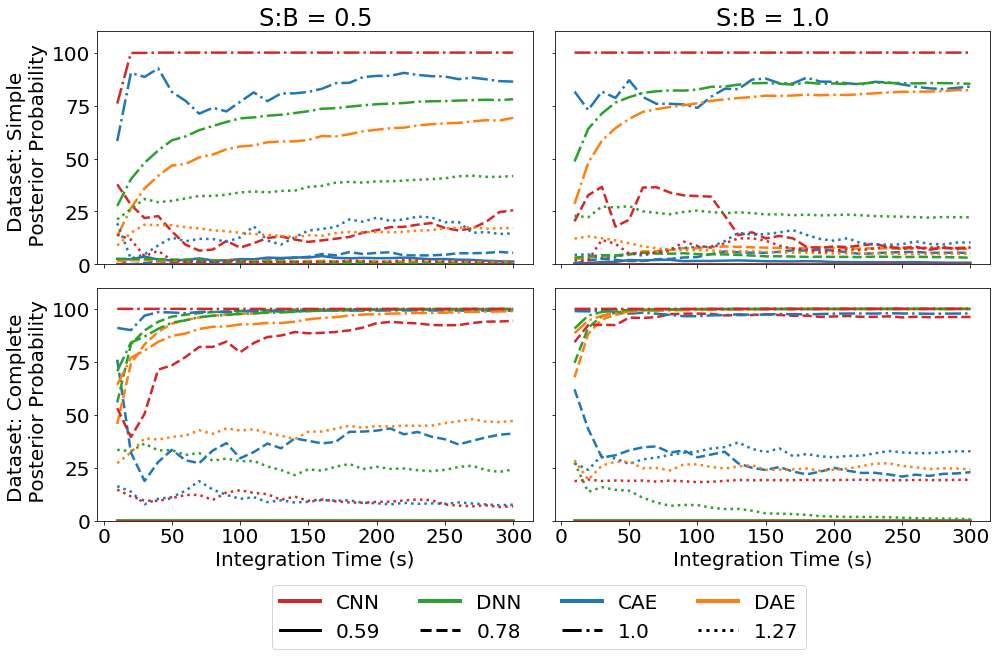
\includegraphics[width=1.0\linewidth]{images/realspectra-cal-cs137}
	\caption{Calibration gain generalization performance in real $^{137}$Cs spectra for the DNN, CNN with and without autoencoder pretraining.}
	\label{fig:realspectra-cal-cs137}
\end{figure}


The figures in \ref{fig:gain_co60} show performance when identifying $^{60}$Co. Some models exhibit improved generalization performance when using the simple dataset over $^{137}$Cs identification. The autoencoders' performance improves for a range of calibrations while the performance of the DNN and CNN improves slightly. The performance of the autoencoders show that pretraining on simulated spectra did have a positive effect on the final network. This also shows that the dense encoding is particularly well suited to changes in calibration.

Performance is degraded when using the full dataset. This is likely due to the models trained on the full dataset assigning higher contributions to other isotopes. Because the spectra for each isotope can look significantly different from each other in the full dataset, the models are more likely to assign higher probabilities to all isotopes.

\begin{figure}[H]
	\centering
	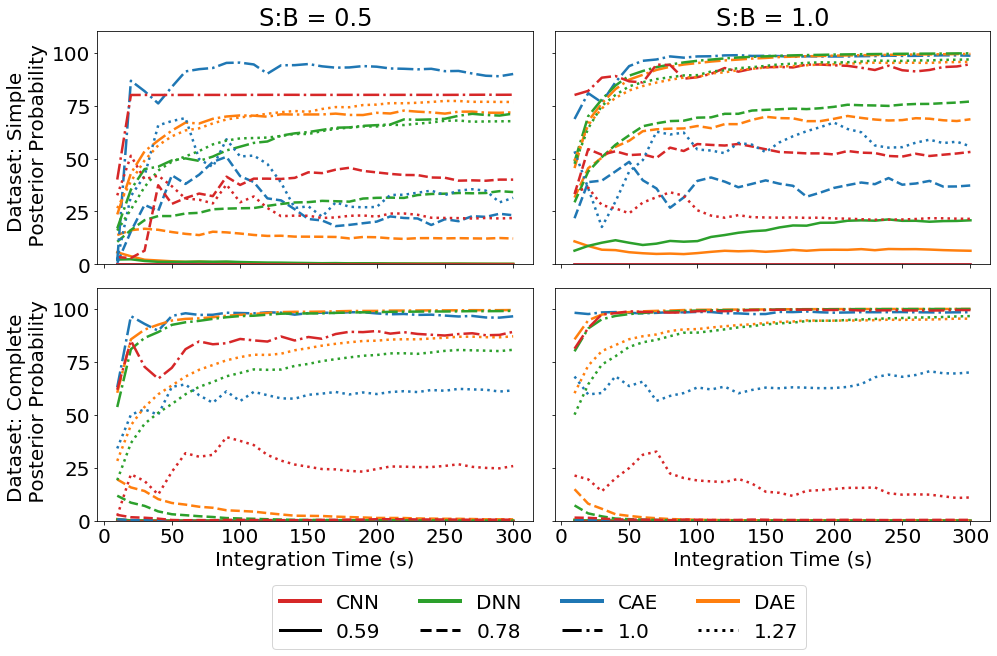
\includegraphics[width=1.0\linewidth]{images/realspectra-cal-co60}
	\caption{Calibration gain generalization performance in real $^{60}$Co spectra for the DNN, CNN with and without autoencoder pretraining.}
	\label{fig:realspectra-cal-co60}
\end{figure}

Subfigures \ref{fig:realspectra-cal-ba133-0-easy} and \ref{fig:realspectra-cal-ba133-1-easy} show that performance on the simple dataset drops significantly when identifying $^{133}$Ba. The drop in performance is attributed to the lack of spectral variety in the simple dataset. For generalization to real spectra, spectral variety in a training set is required for complicated spectra like $^{133}$Ba. Despite this, the models that performed best were convolutional.

Performance improved in complete models. Again, both convolutional models outperformed the purely dense models, with the CNN outperforming the CAE at the higher signal-to-background ratio. All models only generalized to the relative gain settings of 0.78 and 1.0,  


\begin{figure}[H]
	\centering
	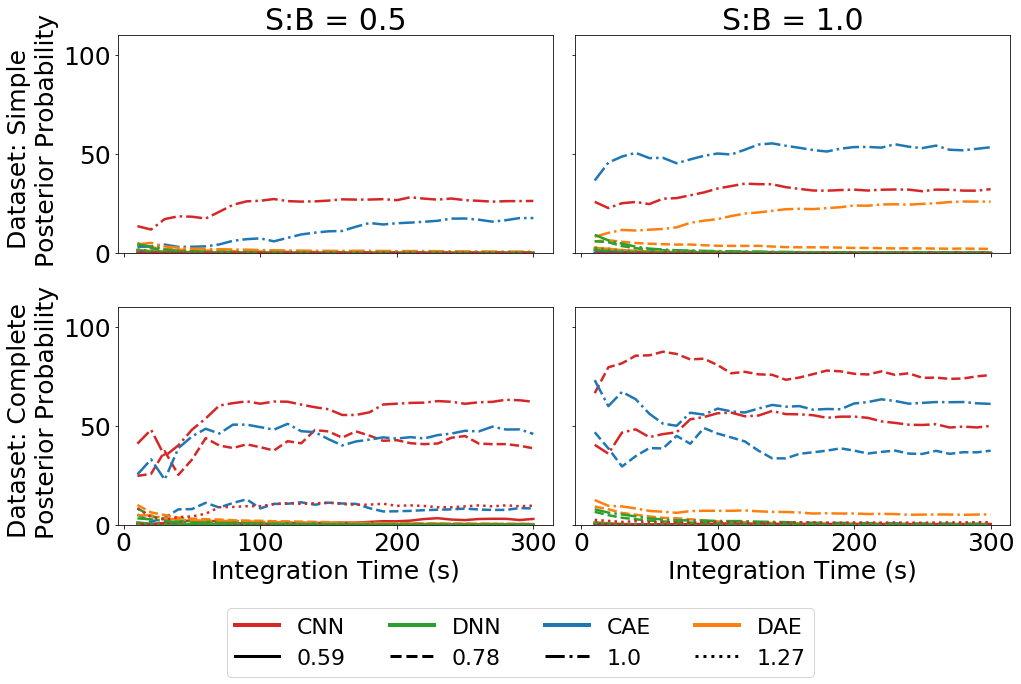
\includegraphics[width=1.0\linewidth]{images/realspectra-cal-ba133}
	\caption{Calibration gain generalization performance in real $^{133}$Ba spectra for the DNN, CNN with and without autoencoder pretraining.}
	\label{fig:realspectra-cal-ba133}
\end{figure}


Figures in \ref{fig:gain_eu152} show performance when identifying $^{152}$Eu. For the first time, convolutional architectures did not outperform the dense models. This performance change only occurred in the simple dataset. As explained above, because of the lack of spectral variety in the simple dataset, generalization to real spectra is more difficult. $^{152}$Eu has many more identifiable photopeaks in a larger range of energies compared to $^{133}$Ba. Because of this, using the channel-based approach (dense architectures) would lead to better performance over approaches that use a form of feature extraction.

The improvement in the convolutional models for $^{152}$Eu identification occurs when more spectral variety is available in the complete dataset. With the complete dataset, all gain settings except 0.59 are identified with high posterior probability above 100 seconds of integration time. 


\begin{figure}[H]
	\centering
	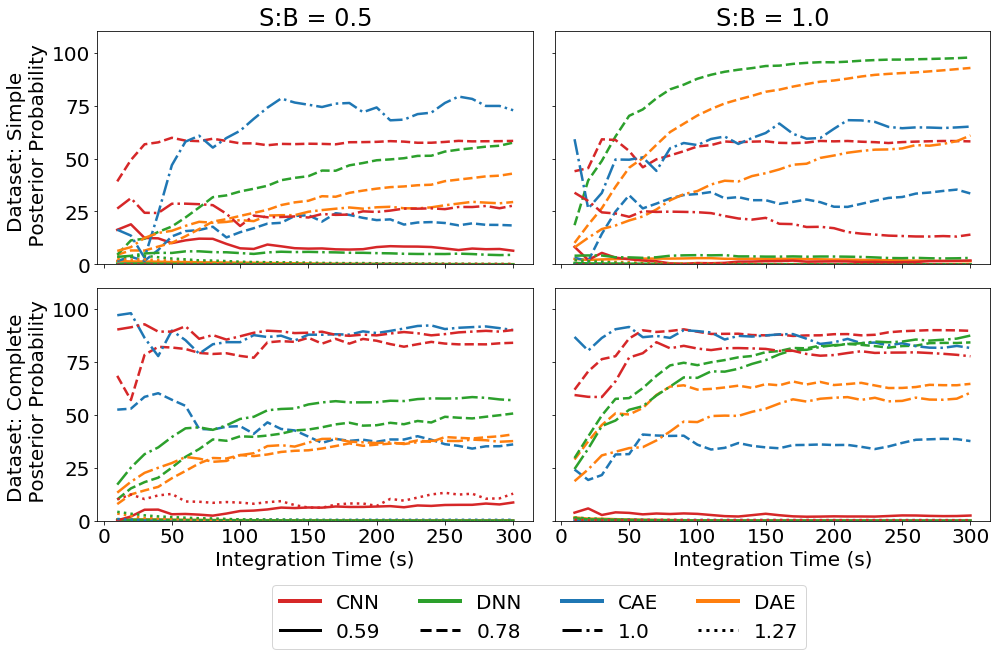
\includegraphics[width=1.0\linewidth]{images/realspectra-cal-eu152}
	\caption{Calibration gain generalization performance in real $^{152}$Eu spectra for the DNN, CNN with and without autoencoder pretraining.}
	\label{fig:realspectra-cal-eu152}
\end{figure}

\subsubsection{Asymptotic Model Performance with Respect to Shielding} \label{real_shielding_performance}

To investigate the generalization performance of the model to increased shielding, spectra of $^{137}$Cs, $^{60}$Co, $^{133}$Ba, and $^{152}$Eu were measured with increasing thicknesses of shielding material. Iron or aluminum blocks were 

Identification performance for $^{137}$Cs was not heavily effected by varying shielding in either training dataset. This is due to shielding not dramatically affecting the single photopeak of $^{137}$Cs. The CNN performs very well in both datasets. The complete DNN performs comparably to complete CNN. The DNN and DAE are affected by increased shielding when trained on the simple dataset, showing that slight changes in spectral shapes affect performance in dense models when they are not exposed to a variety of spectral patterns. When trained on the complete dataset, networks without autoencoder pretraining outperform networks with pretraining.



\begin{figure}[H]
	\centering
	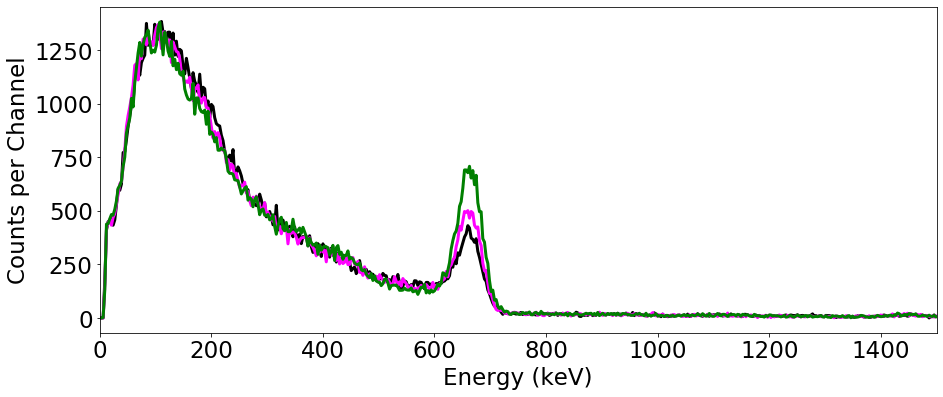
\includegraphics[width=1.0\linewidth]{images/shielded_cs137}
	\caption{Spectra of $^{137}$Cs shielded with increasing amounts of iron.}
	\label{fig:shielded_cs137}
\end{figure}


\begin{figure}[H]
	\centering
	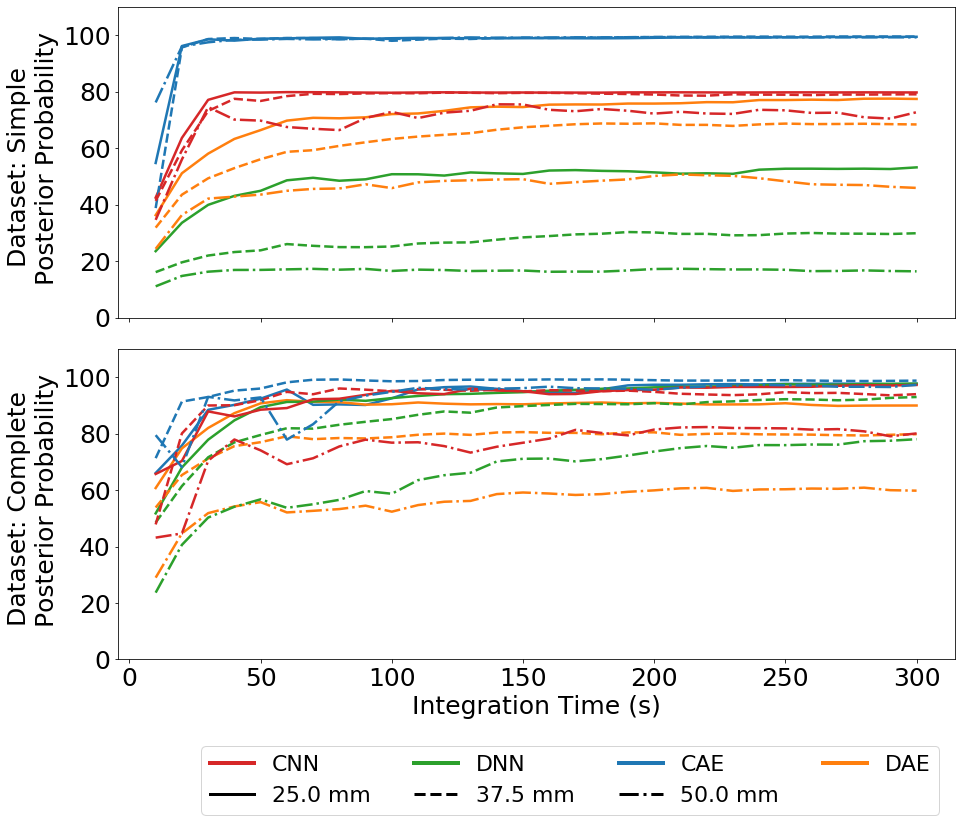
\includegraphics[width=0.9\linewidth]{images/iron_co60}	\caption{Shielding generalization performance in real $^{137}$Cs spectra.}
	\label{fig:iron_cs137}
\end{figure}


The effect of shielding is more significant in $^{60}$Co. As expected, when trained on the simple dataset each model performs worse with heavier shielding. The convolutional models and autoencoders outperform the DNN after 120 seconds of integration time. The DAE performs the best on the highest shielded spectra.  

The DNN is heavily effected by shielding even when trained on the complete dataset. The CNN performs very well, with the DAE performing well over a range of shielding amounts. The DNN was the most drastically affected by the shielding. Compared to the other networks, the DNN has a relatively large variance in its posterior probability for each shielding amount.

\begin{figure}[H]
	\centering
	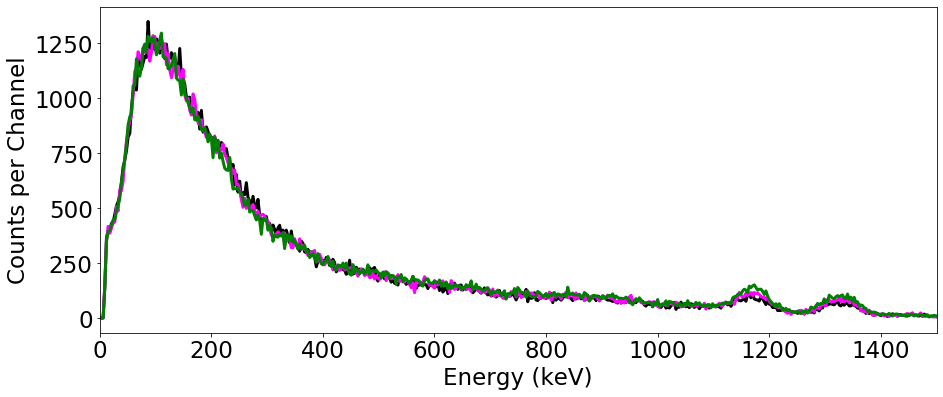
\includegraphics[width=1.0\linewidth]{images/shielded_co60}	\caption{Spectra of $^{60}$Co shielded with increasing amounts of iron.}
	\label{fig:shielded_co60}
\end{figure}

\begin{figure}[H]
	\centering
	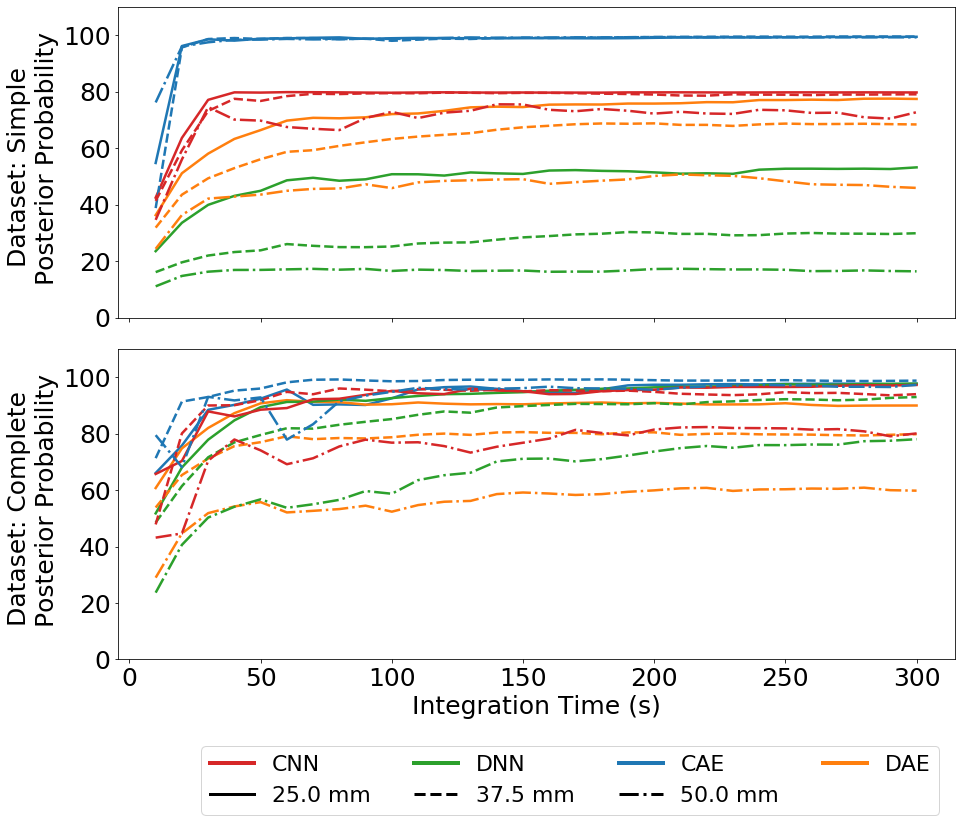
\includegraphics[width=0.9\linewidth]{images/iron_co60}	\caption{Shielding generalization performance in real $^{60}$Co spectra.}
	\label{fig:iron_co60}
\end{figure}


Due to the relatively low gamma-ray energies of $^{133}$Ba compared to the other spectra in this section, aluminum with thicknesses of 6.56 mm, 25.5 mm, and 51.0 mm were used for the light, medium, and heavy settings. When trained on the simple dataset, the CAE performed best. Unlike the previous isotopes, the DAE trained on the simple dataset did not perform well on shielded $^{133}$Ba. Even when trained on the complete dataset, the CAE outperformed the DAE. Characteristic $^{133}$Ba photons have relatively low energy - particularly the photopeaks at 31 and 81 keV. Shielding significantly distorts the spectrum because these photons are easily attenuated. Features like the Compton continuum from the higher energy photopeaks may provide more signal when identifying these isotopes in shielded case. These features are also better exploited in the networks trained on the complete dataset. The dense architectures perform poorly even when trained on the complete dataset. The variance of the posterior probability for the convolutional architectures are lower than the DAE, showing they are more consistent.


\begin{figure}[H]
	\centering
	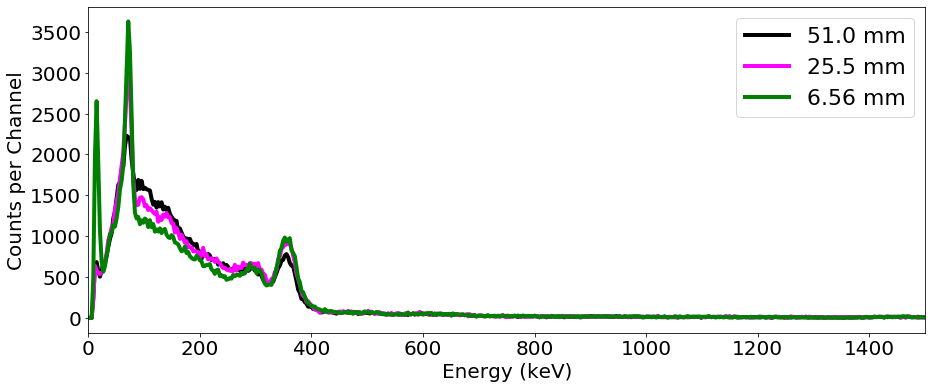
\includegraphics[width=1.0\linewidth]{images/shielded_ba133}	\caption{Spectra of $^{133}$Ba shielded with increasing amounts of aluminum.}
	\label{fig:shielded_ba133}
\end{figure}

\begin{figure}[H]
	\centering
	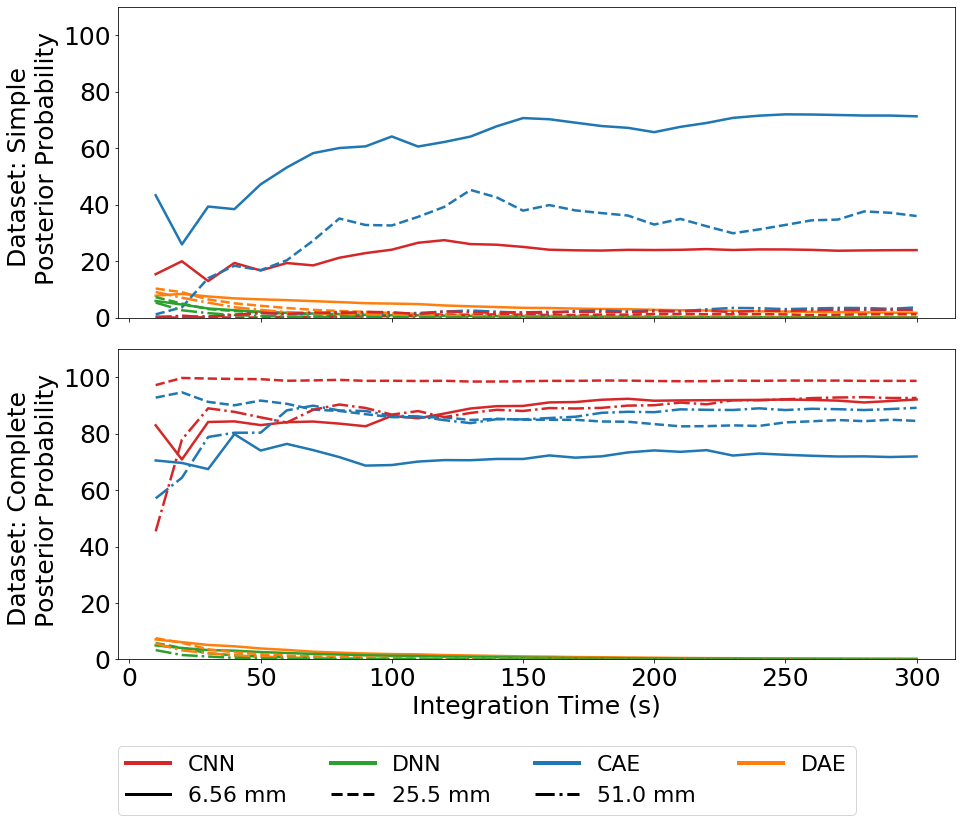
\includegraphics[width=0.9\linewidth]{images/alum_ba133}	\caption{Shielding generalization performance in real $^{133}$Ba spectra.}
	\label{fig:alum_ba133}
\end{figure}



The simple DAE performs well generalizing to shielded $^{152}$Eu while the simple CNN generalizes poorly. The simple CAE and DNN both perform similarly across the full range of shielding. 

The complete CNN identifies lightly and moderately shielded $^{152}$Eu with a high posterior probability. The DNN performs second best, identifying these spectra with a slightly lower posterior probability. The complete DNN operates consistently over a range of integration times for the heavily shielded $^{152}$Eu. Only after 150 seconds of integration time does the CNN perform similarly on heavily shielded $^{152}$Eu. % The complete CAE performs worse.



\begin{figure}[H]
	\centering
	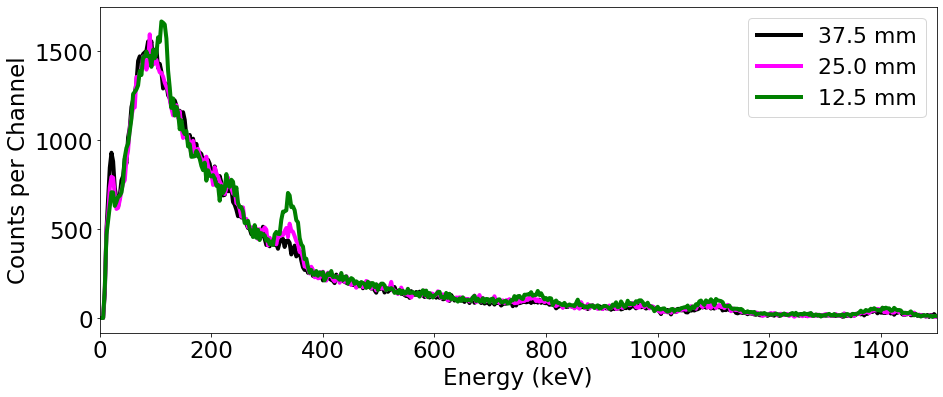
\includegraphics[width=1.0\linewidth]{images/shielded_eu152}
	\caption{Spectra of $^{152}$Eu shielded with increasing amounts of iron.}
	\label{fig:shielded_eu152}
\end{figure}


\begin{figure}[H]
	\centering
	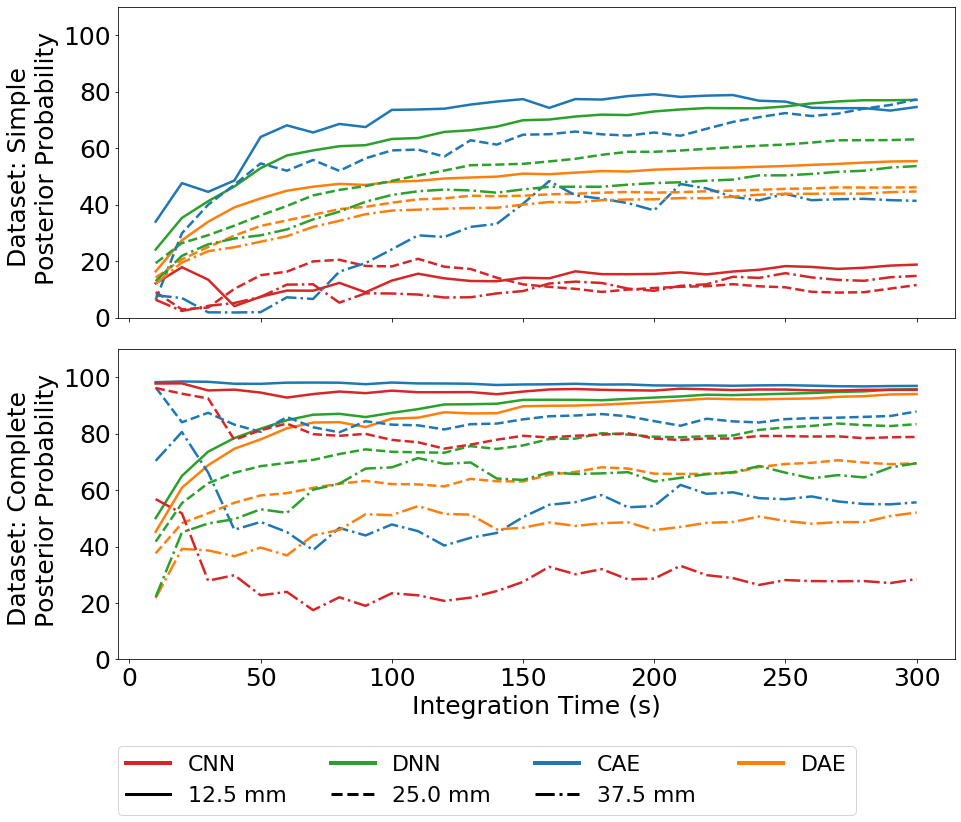
\includegraphics[width=0.9\linewidth]{images/iron_eu152}	\caption{Shielding generalization performance in real $^{152}$Eu spectra.}
	\label{fig:iron_eu152}
\end{figure}

\section{Chapter Discussion and Conclusion}

This chapter shows that CNNs trained on the complete dataset generalize very well to simulated and real gamma-ray spectra. When trained on the simple dataset CNNs often also perform well when identifying spectra outside the simple dataset's parameters, but struggle with real spectra. The autoencoders perform poorly in the simulated spectra, but generalize well to parameters outside the simple training set - particularly DAEs. There is also some evidence that CAEs generalize better to isotopes with predominately low energy photopeaks in real spectra. Occasionally, at the lower signal-to-background ratio, the DNN outperforms the CNN. Because the dense architecture is more suited to comparing counts in different regions, it should be more robust against changes in Compton continua as it compares counts in photopeak areas. Despite this, DNN's offer unpredictable performance. Due to the large number of inputs, the DNN's are likely overtraining to specific combinations of noise in the training datasets.

In addition to the above, the results also shown that using datasets of fixed sizes should be preferred over using online data augmentation. Online data augmentation usually reduced performance in each network. There is some evidence that the CNN generalizes better when trained with online data augmentation. This may be due to the larger capacity of the CNN compared to the DNN. 

% To take advantage of this, it may be best to include a committee of CNN's and DNN's, or to train networks for specific ranges of integration time.

% A committee of models can be constructed with CAEs, DAEs, and CNNs. 



